\documentclass[12pt]{article}
\usepackage{amsfonts, amssymb, amsmath, amsthm}
\usepackage[margin=1in]{geometry}
\usepackage{tikz}
\usetikzlibrary{patterns, decorations.pathreplacing, arrows.meta}

\pagestyle{myheadings}
\markright{Explainer: Equivalence of Connectedness Definitions\hfill}

\newcommand{\R}{\mathbb{R}}

\begin{document}

\begin{center}
    \textbf{\Large Two Faces of Connectedness}\\[0.5em]
    \large Why the separated-sets and relative-open definitions agree
\end{center}

\section{The Two Definitions}

Both definitions capture the idea that a connected set is ``one piece,'' but they phrase it differently.

\subsection{Definition 1: Separated Sets (Rudin's Definition)}

$E$ is \textbf{disconnected} if $E = A \cup B$ where $A, B$ are nonempty and \textbf{separated}:
\[
\overline{A} \cap B = \varnothing \quad \text{and} \quad A \cap \overline{B} = \varnothing
\]

\begin{center}
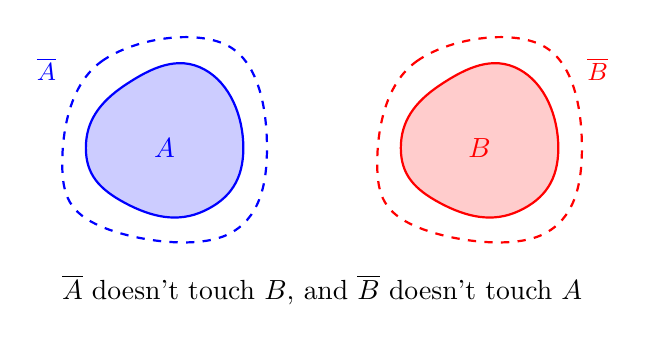
\begin{tikzpicture}[scale=1]
    % Set A with its closure
    \draw[blue, thick, fill=blue!20] plot[smooth cycle, tension=0.8]
        coordinates {(-3,0) (-2.5,0.8) (-1.5,1) (-1,0) (-1.5,-0.8) (-2.5,-0.7)};
    \draw[blue, dashed, thick] plot[smooth cycle, tension=0.7]
        coordinates {(-3.3,-0.2) (-2.8,1.1) (-1.2,1.3) (-0.7,0) (-1.2,-1.1) (-2.8,-1)};
    \node[blue] at (-2, 0) {$A$};
    \node[blue, font=\small] at (-3.5, 1) {$\overline{A}$};

    % Set B with its closure
    \draw[red, thick, fill=red!20] plot[smooth cycle, tension=0.8]
        coordinates {(1,0) (1.5,0.8) (2.5,1) (3,0) (2.5,-0.8) (1.5,-0.7)};
    \draw[red, dashed, thick] plot[smooth cycle, tension=0.7]
        coordinates {(0.7,-0.2) (1.2,1.1) (2.8,1.3) (3.3,0) (2.8,-1.1) (1.2,-1)};
    \node[red] at (2, 0) {$B$};
    \node[red, font=\small] at (3.5, 1) {$\overline{B}$};

    \node at (0, -1.8) {$\overline{A}$ doesn't touch $B$, and $\overline{B}$ doesn't touch $A$};
\end{tikzpicture}
\end{center}

\subsection{Definition 2: Relative Open Sets}

$E$ is \textbf{disconnected} if $E = A \cup B$ where $A, B$ are nonempty, disjoint, and both \textbf{open relative to $E$}.

\begin{center}
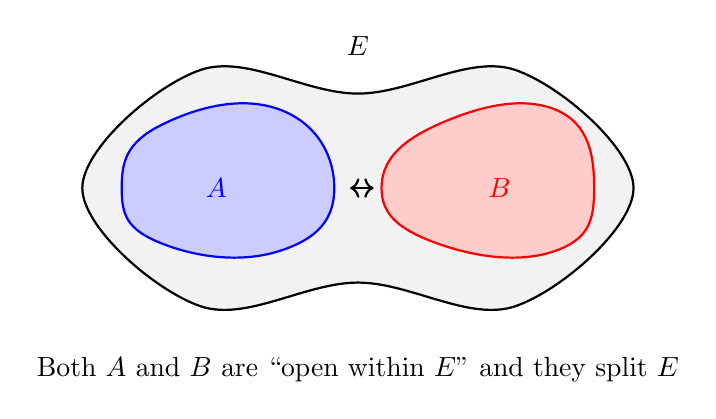
\begin{tikzpicture}[scale=1]
    % The set E as a big region
    \draw[thick, fill=gray!10] plot[smooth cycle, tension=0.6]
        coordinates {(-3.5,0) (-2,1.5) (0,1.2) (2,1.5) (3.5,0) (2,-1.5) (0,-1.2) (-2,-1.5)};
    \node at (0, 1.8) {$E$};

    % A - open relative to E
    \draw[blue, thick, fill=blue!20] plot[smooth cycle, tension=0.8]
        coordinates {(-3,0) (-2.5,0.8) (-1,1) (-0.3,0) (-1,-0.8) (-2.5,-0.7)};
    \node[blue] at (-1.8, 0) {$A$};

    % B - open relative to E
    \draw[red, thick, fill=red!20] plot[smooth cycle, tension=0.8]
        coordinates {(0.3,0) (1,0.8) (2.5,1) (3,0) (2.5,-0.8) (1,-0.7)};
    \node[red] at (1.8, 0) {$B$};

    % Gap
    \draw[<->, thick] (-0.1, 0) -- (0.2, 0);

    \node at (0, -2.3) {Both $A$ and $B$ are ``open within $E$'' and they split $E$};
\end{tikzpicture}
\end{center}

\section{What Does ``Open Relative to $E$'' Mean?}

$A$ is \textbf{open relative to $E$} if every point of $A$ has a neighborhood (within $E$) contained in $A$.

\begin{center}
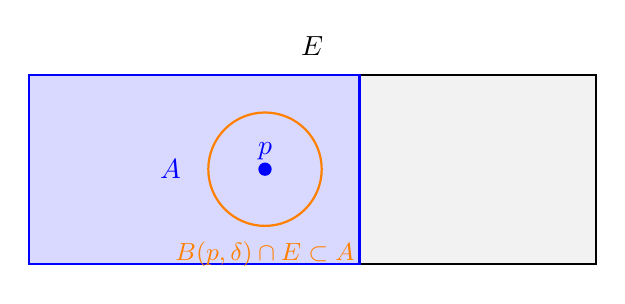
\begin{tikzpicture}[scale=1.2]
    % E
    \draw[thick, fill=gray!10] (-3, -1) rectangle (3, 1);
    \node at (0, 1.3) {$E$};

    % A (left half, open relative to E)
    \draw[blue, thick, fill=blue!15] (-3, -1) rectangle (0.5, 1);
    \node[blue] at (-1.5, 0) {$A$};

    % A point in A
    \fill[blue] (-0.5, 0) circle (2pt) node[above] {$p$};

    % Ball around p stays in A (within E)
    \draw[orange, thick] (-0.5, 0) circle (0.6);
    \node[orange, font=\small] at (-0.5, -0.9) {$B(p, \delta) \cap E \subset A$};
\end{tikzpicture}
\end{center}

Equivalently, $A$ is open relative to $E$ if $A = E \cap U$ for some open set $U$ in the ambient space.

\section{Why Are These Definitions Equivalent?}

\subsection{Direction 1: Separated $\Rightarrow$ Relatively Open}

If $\overline{A} \cap B = \varnothing$ and $A \cap \overline{B} = \varnothing$:

\begin{center}
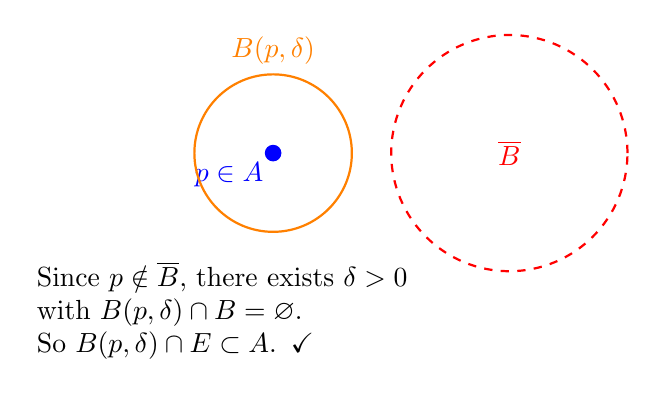
\begin{tikzpicture}[scale=1]
    % Point in A
    \fill[blue] (0, 0) circle (3pt) node[below left] {$p \in A$};

    % Since A cap closure(B) = empty, p is not in closure(B)
    \draw[red, dashed, thick] (3, 0) circle (1.5);
    \node[red] at (3, 0) {$\overline{B}$};

    % p is outside closure(B), so there's a delta ball missing B
    \draw[orange, thick] (0, 0) circle (1);
    \node[orange] at (0, 1.3) {$B(p, \delta)$};

    \node[text width=6cm, align=left] at (0, -2) {
        Since $p \notin \overline{B}$, there exists $\delta > 0$\\
        with $B(p, \delta) \cap B = \varnothing$.\\
        So $B(p, \delta) \cap E \subset A$. \checkmark
    };
\end{tikzpicture}
\end{center}

\textbf{Key idea:} ``$A \cap \overline{B} = \varnothing$'' means every point of $A$ is at positive distance from $B$, so $A$ is open relative to $E$. By symmetry, $B$ is also open relative to $E$.

\subsection{Direction 2: Relatively Open $\Rightarrow$ Separated}

If $A, B$ are both open relative to $E$, disjoint, and $A \cup B = E$:

\begin{center}
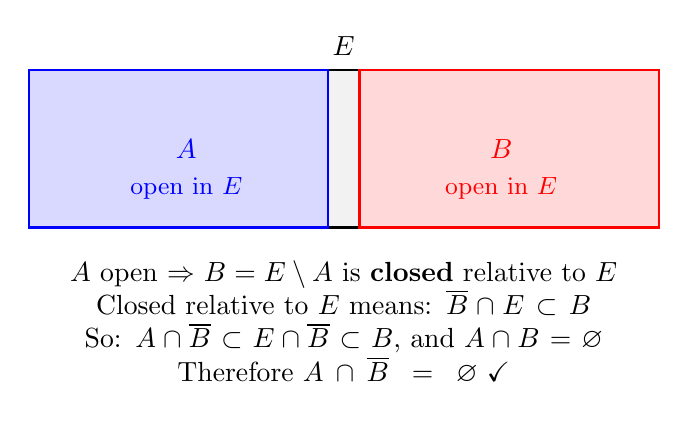
\begin{tikzpicture}[scale=1]
    \draw[thick, fill=gray!10] (-4, -1) rectangle (4, 1);
    \node at (0, 1.3) {$E$};

    % A open in E
    \draw[blue, thick, fill=blue!15] (-4, -1) rectangle (-0.2, 1);
    \node[blue] at (-2, 0) {$A$};
    \node[blue, font=\small] at (-2, -0.5) {open in $E$};

    % B open in E
    \draw[red, thick, fill=red!15] (0.2, -1) rectangle (4, 1);
    \node[red] at (2, 0) {$B$};
    \node[red, font=\small] at (2, -0.5) {open in $E$};

    \node[text width=7cm, align=center] at (0, -2.2) {
        $A$ open $\Rightarrow$ $B = E \setminus A$ is \textbf{closed} relative to $E$\\
        Closed relative to $E$ means: $\overline{B} \cap E \subset B$\\
        So: $A \cap \overline{B} \subset E \cap \overline{B} \subset B$, and $A \cap B = \varnothing$\\
        Therefore $A \cap \overline{B} = \varnothing$ \checkmark
    };
\end{tikzpicture}
\end{center}

\textbf{Key idea:} If $A$ is open in $E$, then $B = E \setminus A$ is closed in $E$, meaning $\overline{B} \cap E \subset B$. So $A$ can't touch $\overline{B}$ (within $E$, and $A \subset E$). By symmetry, $B$ can't touch $\overline{A}$.

\section{The Open/Closed Duality}

The magic ingredient: when $E = A \cup B$ with $A \cap B = \varnothing$:
\[
A \text{ open in } E \iff B = E \setminus A \text{ closed in } E
\]

So if \emph{both} $A$ and $B$ are open in $E$, then both are \emph{also} closed in $E$! This ``clopen'' property is what makes them separated.

\begin{center}
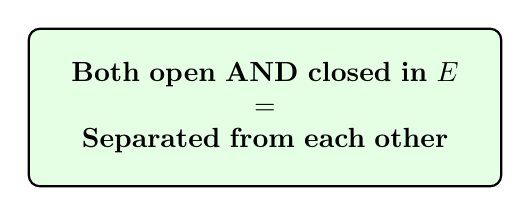
\begin{tikzpicture}
    \draw[thick, rounded corners, fill=green!10] (-3, -1) rectangle (3, 1);
    \node[text width=5.5cm, align=center] at (0, 0) {
        \textbf{Both open AND closed in $E$}\\
        $=$\\
        \textbf{Separated from each other}
    };
\end{tikzpicture}
\end{center}

\section{Summary}

\begin{center}
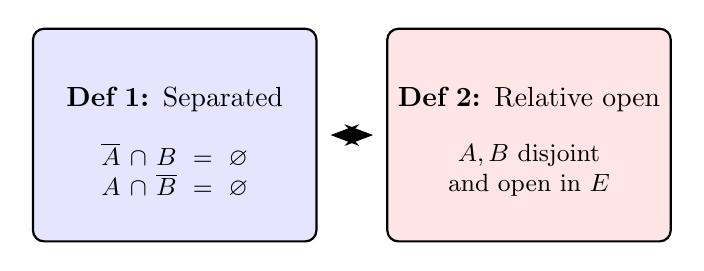
\begin{tikzpicture}[scale=0.9]
    % Definition 1
    \draw[thick, rounded corners, fill=blue!10] (-4.5, -1.5) rectangle (-0.5, 1.5);
    \node[text width=3.5cm, align=center] at (-2.5, 0.5) {\textbf{Def 1:} Separated};
    \node[text width=3.5cm, align=center, font=\small] at (-2.5, -0.5) {$\overline{A} \cap B = \varnothing$\\$A \cap \overline{B} = \varnothing$};

    % Definition 2
    \draw[thick, rounded corners, fill=red!10] (0.5, -1.5) rectangle (4.5, 1.5);
    \node[text width=3.5cm, align=center] at (2.5, 0.5) {\textbf{Def 2:} Relative open};
    \node[text width=3.5cm, align=center, font=\small] at (2.5, -0.5) {$A, B$ disjoint\\and open in $E$};

    % Double arrow
    \draw[{Stealth}-{Stealth}, ultra thick] (-0.3, 0) -- (0.3, 0);
\end{tikzpicture}
\end{center}

The bridge between them: \textbf{relative closure}. In a disjoint partition $E = A \cup B$:
\begin{itemize}
    \item Separated $\Rightarrow$ each piece avoids the other's closure $\Rightarrow$ each piece is open in $E$
    \item Relatively open $\Rightarrow$ each piece is also closed in $E$ $\Rightarrow$ separated
\end{itemize}

\end{document}
